\setAuthor{Taavet Kalda}
\setRound{lahtine}
\setYear{2020}
\setNumber{G 6}
\setDifficulty{6}
\setTopic{TODO}

\prob{Kondensaatorid}
\begin{wrapfigure}[8]{r}{0.3\linewidth}
		\vspace{-5pt}
		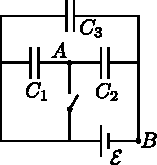
\includegraphics[width=\linewidth]{2020-lahg-06-yl.pdf}
	\end{wrapfigure}
	Pingeallikas pingega $\mathcal E$ on ühendatud kolme kondensaatoriga mahtuvustega $C_1$, $C_2$ ja $C_3$. Alguses hoitakse lüliti pikalt kinnises olekus. Mitu korda muutub punktide $A$ ja $B$ vaheline pinge peale lüliti avamist ja pika aja möödumist? 
	
	
	
\hint

\solu
Peale lüliti avamist pole punkt $A$ enam ülejäänud skeemiga juhtmete kaudu ühendatud. Kuna laengud ei saa läbi õhu hüpata (pinged on läbilöögitugevusest palju väiksemad), kehtib skeemi $A$ poolses osas laengu jäävus.

Alguses on $A$ ja $B$ vaheline pinge $V_1 = \mathcal E$. Punkti $A$ suhtes on $C_1$ ja $C_2$ pinged vastavalt \SI{0}{V} ja $\mathcal E$. Järelikult on $C_1$ ja $C_2$ sisemiste plaatide kogulaeng $q_\mathrm{tot} = 0 + C_2\mathcal E = C_2\mathcal E$.

Olgu punktide $A$ ja $B$ vaheline pinge peale lüliti avamist $V_2$. $C_1$ ja $C_2$ pinged punkti $A$ suhtes on siis $V_2 - \mathcal E$ ning $V_2$ ja sisemiste plaatide kogulaeng on $q_\mathrm{tot} = C_1(V_2 - \mathcal E) + C_2V_2$. Kokkuvõttes saame
\[
q_\mathrm{tot} = C_2\mathcal E = C_1(V_2 - \mathcal E) + C_2V_2,
\]
millest $V_2=\mathcal E$. Näeme, et pinge punktide $A$ ja $B$ vahel ei muutu.
\probend